\documentclass[a4paper, 11pt]{scrartcl}
\usepackage[utf8]{inputenc}
\usepackage[english]{babel}
\usepackage[T1]{fontenc}
\usepackage{amsmath}
\usepackage{graphicx}
\usepackage{url}
\usepackage{float}
\usepackage{fancyhdr}
\bibliographystyle{plainnat}
\newcommand{\uproman}[1]{\uppercase\expandafter{\romannumeral#1}}

\title {Development and construction of a 2D Laser Scanner}
\author {Niklas H}
\date {\today}

\begin{document}
\maketitle
\tableofcontents
\newpage
\section{Introduction}
Many laser scanning systems for material processing today are based on galvanometer-actuated mirror systems and utilize fiber lasers ($\lambda = 1064nm$) for efficient and fast engraving on metals. However, galvanometers are expensive and complicated to drive.  This projects goal is to create a similar system using stepper motors, which are very simple to use and laser diodes ($\lambda=650nm$ and $\lambda=445nm$). The secondary goal is to create a cheap but accurate drive system which should be possible to build with minimal tools (3D-Printer, lathe (optional) and basic soldering equipment) from scratch. For this sake, two versions will be built, the first one utilizing a low power laser diode and no f-theta lens for a safe proof-of-concept and the second one utilizing a high-power laser diode for engraving. \\
In this documentation, the mechanical, electrical, mathematical and programming side of the project will be discussed.

\section{Theory}
In this section, relevant theory will be discussed. The development of the scanner will be based on these details. \\
\subsection{Laser diodes} 
Laser diodes are special semiconductors that emit spatially coherent and monochromatic light of a specific wavelength $\lambda$ (laser beam). Laser diodes are relatively fragile components which electrically behave similar to normal diodes, meaning low resistance in one current direction and high resistance in the opposite direction. For laser diodes to work properly, they must be driven with a constant current\footnote{Laser diodes are easily damaged by current spikes or excess heat}. Therefore, it is good practice to use constant current sources and heatsinks for driving laserdiodes. Also, laser diodes oftentimes emit laser beams with relatively high divergence, so a collimator is required in order to reduce the divergence to a few $mrad$. 

\subsection{Stepper motors}
Stepper motors reach high positioning accuracy by performing movements in discrete steps (usually $1.8^\circ$). The appropriate winding currents are supplied by stepper motor drivers. These drivers are given two signals: STEP and DIR. One STEP pulse from the controller advances the motor position one step, whilst the DIR signal (low or high) indicates the direction. The accuracy can be improved by using special drivers which interpolate the rotation between poles (micro-stepping). 

\subsection{Optics of the scanner} 
\begin{figure}[H]
\begin{center}
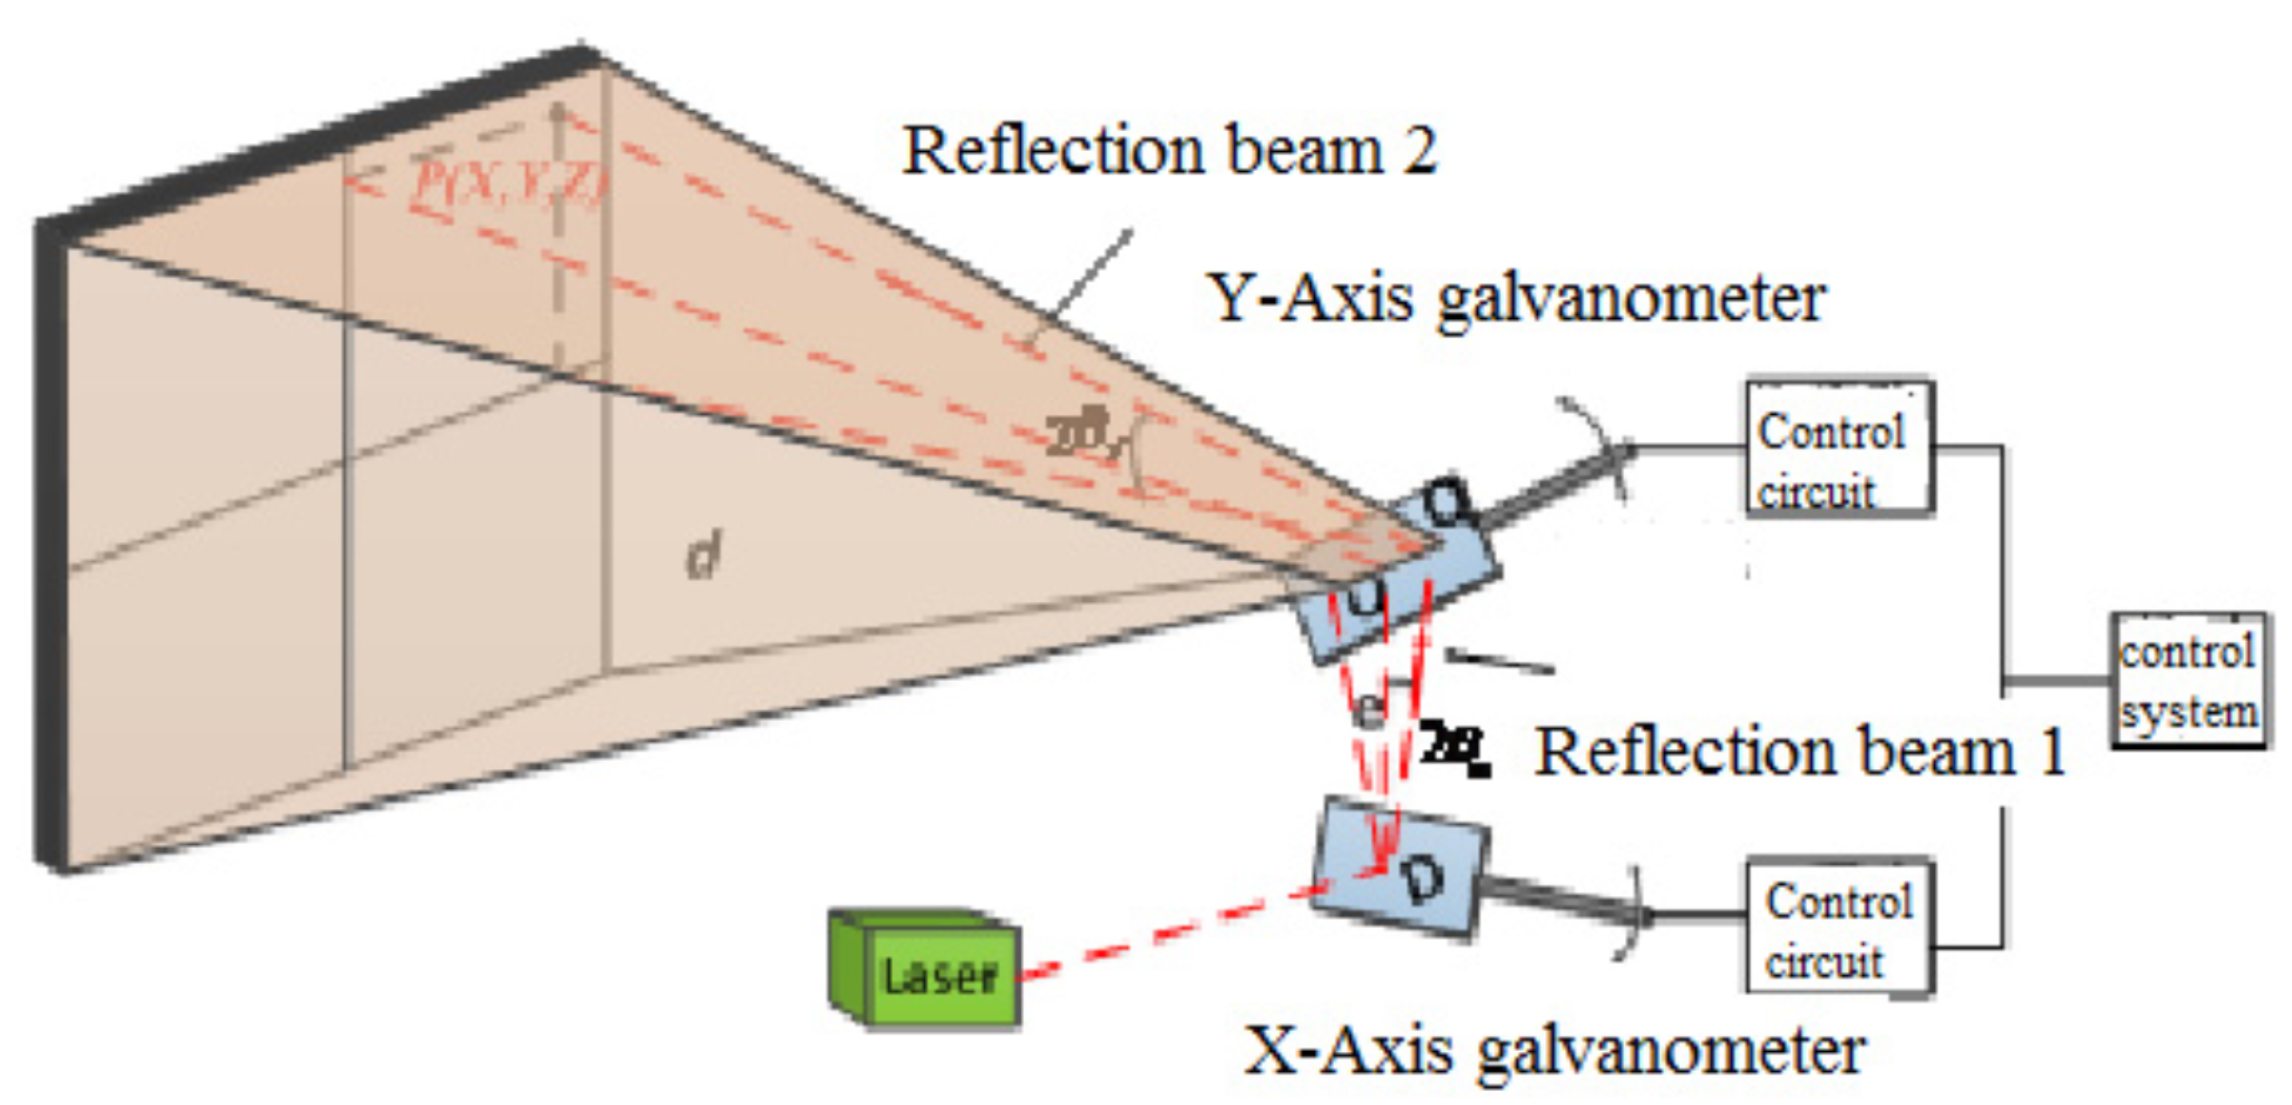
\includegraphics[width=15cm]{img/optics.png}
\caption{Model of the optical mirror system \cite{Meng.2019}}
\label{optics}
\end{center}
\end{figure}
Because the scanner can only indirectly control the laser dot on the working plane by turning its mirrors, some sort of mathematical representation of this system must be derived. This representation will used for turning XY-directions into mirror rotation angles. From \cite{Meng.2019} we get the following equations:
\begin{equation}\label{eqn1}
x=e\cdot tan(2\theta_x)+tan(2\theta_x) \cdot \sqrt{d^2+y^2} 
\end{equation} 
\begin{equation}\label{eqn2}
y = d\cdot tan(\theta_y)
\end{equation} 
where $x$ and $y$ are the point coordinates on the plane, $\theta_x$ and $\theta_y$ are the rotations angles of the mirrors\footnote{More specifically: $\theta_x$ is the angle between the laser beam and the first reflection beam minus $90^\circ$. Similarly, $\theta_y$ is the angle between the first and second reflection beam minus $90^\circ$.}, $e$ is the vertical distance between the mirror axes and $d$ is the normal distance between the projection plane and the Y-mirror rotation axis. \\
Since $x$ and $y$ are given by the user (rather the gcode), equations \ref{eqn1} and \ref{eqn2} must be solved for $\theta_x$ and $\theta_y$. These angles will be turned into step signals for the steppers. From equation \ref{eqn2} we can derive 
\begin{equation}\label{eqn3}
\theta_y = \frac{arctan(\frac{y}{d})}{2}
\end{equation} 
From equation \ref{eqn1}, $\theta_x$ can be found:
\begin{equation}\label{eqn4}
\theta_x=\frac{arctan\left( \frac{x}{e+\sqrt{d^2+y^2}}\right) }{2}
\end{equation}
Looking at figure \ref{optics}, $x$ and $y$ must be zero, when $\theta_x=theta_y=0^\circ$ \footnote{with these angles, all beams are orthogonal. This configuration is referred to the neutral or home position.}. Equations \ref{eqn3} and \ref{eqn4} confirm this. 

\section{Implementation}
In this section, construction details of the galvo scanner will be explained.
\subsection{Mechanics and Optics}
\begin{figure}[H]
\begin{center}
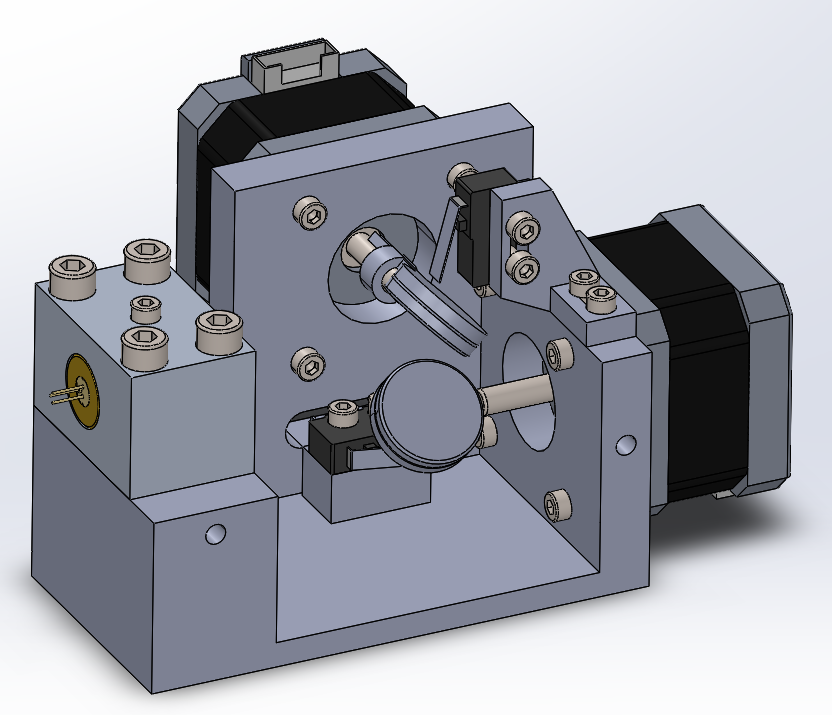
\includegraphics[width=15cm]{img/mechanics.png}
\caption{CAD-Rendering of the mechanical system}
\label{mechanics}
\end{center}
\end{figure}
The mechanics of this design are relatively simple: The mirrors are attached to stepper motors which are screwed onto the 3D-printed base. This base also has features to screw on endswitches (for homing the mirrors) and the laserdiode array. The latter consists of a machined aluminum block into which the laserdiode holder (machined brass) fits. This holder also has a M9x0.5 thread for the collimator unit. The collimator can be adjusted via this thread.
\subsection{Electronics}
\begin{figure}[H]
\begin{center}
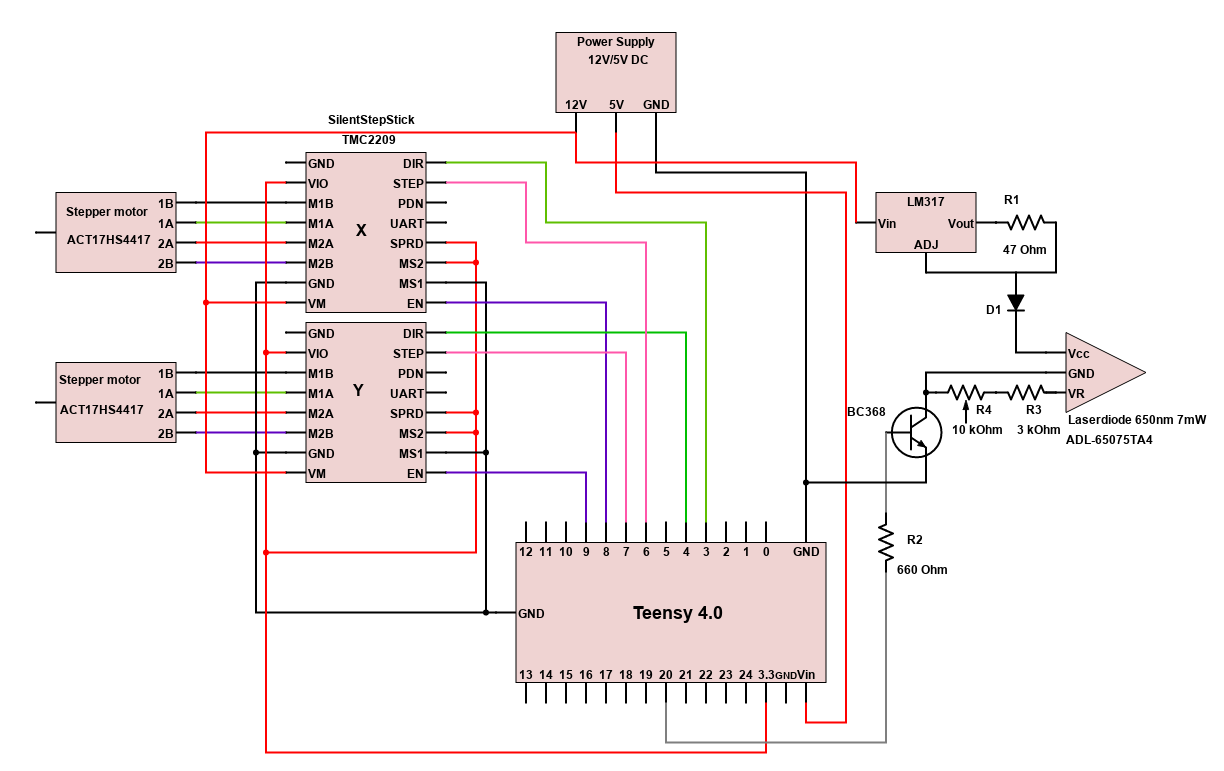
\includegraphics[width=15cm]{img/electronics.png}
\caption{Wiring diagram for the system}
\label{electronics}
\end{center}
\end{figure}
Figure \ref{electronics} shows the electrical diagram of the system. The Stepper motors are Nema-17 ACT 17hs4417 steppers. The SilentStepSticks (containing Trinamic TMC2209 ICs)  were chosen as drivers because of their high micro-stepping capabilities (up to 256), extremely low noise and relatively low cost (about 10 Euros/driver). \\
For the main controller, a Teensy 4.0 was chosen because of the extremely high clock frequency of 600Mhz\footnote{In comparison, an Arduino Nano only has 16MHz clock frequency!} and its easy programmability through the Arduino IDE. It must be noted, that the Teensy 4.0 only tolerates 3.3V logic voltage. 

\paragraph{Note:} Teensy Boards and laserdiodes can be very fragile electrical components (multiple Teensies and Diodes were destroyed in this project), so it may be worth the money and effort to use an Arduino (Nano in this case) in order to test the circuits/code and use dummy loads for simulating laser diodes. Since the SilentStepStick-Drivers can tolerate 3.3V and 5V as logic voltages, the microcontrollers can be changed without changing the circuit. However, the footprints are not equal, so jumper cables are necessary for replacing the Teensy with an Arduino. \\

For driving the laserdiode, a special diode driver is used, which can supply 0-500mA of constant regulated current\footnote{It is possible to use a LM317 and correct resistors for a constant current source. This was tested in this project, but resulted in a lot of destroyed laser diodes, which is why a complete driver circuit was bought.}. \\
This driver circuit is activated by a NPN-Transistor (specifially, a BC368). For calculating its base restistance $R_2$, a base current of the BC368 transistor of $I_B=5mA$ is selected \cite[p. 3]{SemiconductorComponentsIndustries.2007}. Since the Teensy 4.0 logic voltage is $3.3V$, a resistance value of $R_2=\frac{3.3V}{5mA}=660\Omega$ is selected. \\
The Laser diode has three pins: \textit{Vcc}, \textit{GND} and \textit{VR}. \textit{Vcc} is connected to the output of the constant current source, \textit{GND} is connected to the Collector of the transistor to switch it on or off. \textit{VR} is left unconnected. 
For supplying Vcc (5V) for the Teensy and the laser driver, a LM317 linear voltage regulator is used in the shown configuration. The resistors $R_1$ and $R_2$ can be computed as follows \cite[p. 10]{lm317}: 
\begin{equation}
V_{out} = 1.25 \cdot \left( 1+\frac{R_2}{R_1} \right)
\end{equation}
$V_{out}$ must be 5V and $R_1$ is chosen to be $1k\Omega$. Therefore, $R_2$ must be:
\begin{equation}
R_2 = \left( \frac{V_{out}}{1.25V} - 1 \right) \cdot R_1 =  \left( \frac{5V}{1.25V} - 1 \right) \cdot 1000\Omega = 3000\Omega
\end{equation}
$R_4$ and $R_5$ are pull-down resistors that draw the pin state of pins $9$ and $10$ (pins for the endstops) to the low state. \\
$JP_1$ and $JP_2$ are jumpers that set the microstepping mode of the stepper motor drivers to $\frac{1}{8}$ (jumper disconnected) or $\frac{1}{64}$ (jumper connected).
\subsection{Code}
\begin{figure}[H]
\begin{center}
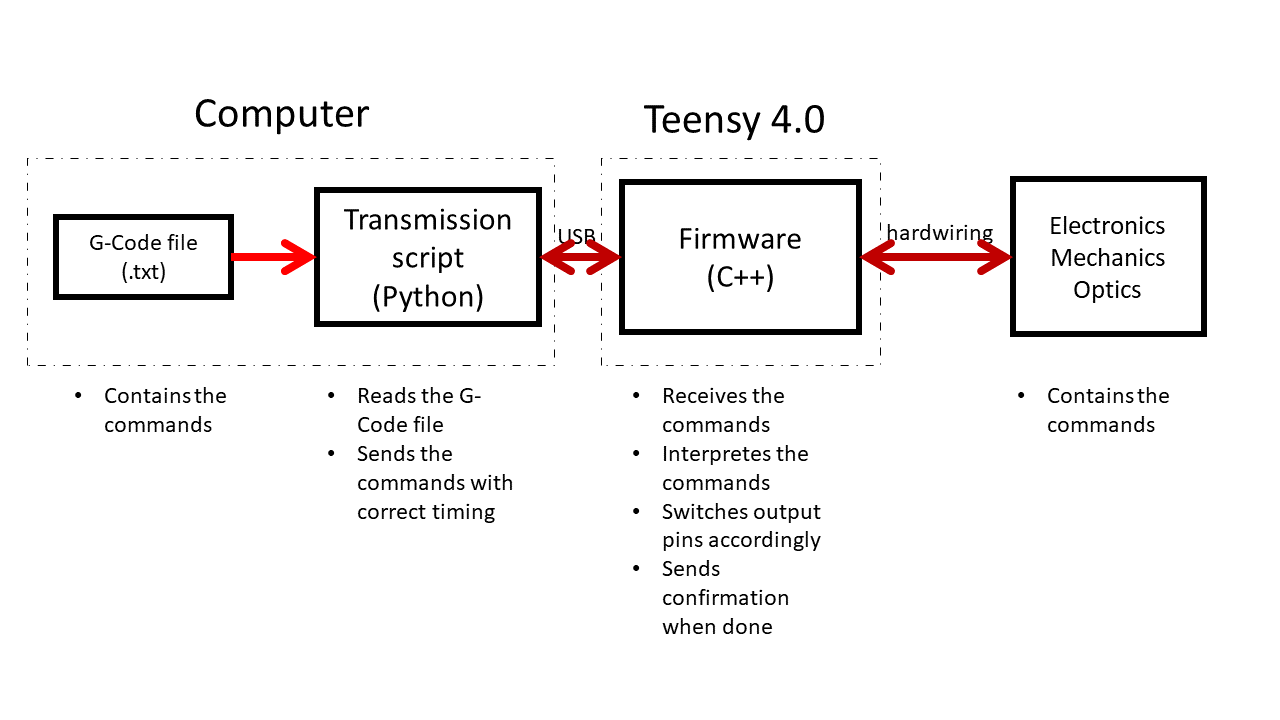
\includegraphics[width=15cm]{img/programArchitecture.png}
\caption{A simplified diagram of the program architecture}
\label{code}
\end{center}
\end{figure}
The programm architecture (see figure \ref{code}) consists of three main parts: The teensy firmware, a python script for Gcode transmission and the G-Code itself. 
\paragraph{Firmware}
The firmware is the most critical part of the architecture: It interpretes the received (via Serial) G-Code commands and coordinates all of the outputs and inputs, such as step and direction signals and the transistor base for the laser or the endstop signals. Because it is directly compiled onto the Teensy via the Arduino IDE, it is written in C++.\\
The firmware supports the following G-Code commands: G0, G1, G2, G3, G28, G60, G61, M3, M4, M5, M201, M203. \footnote{For a detailled explanation and syntax details, see the GalvoStep wiki at \url{https://github.com/NiklasHammerstone/GalvoStep}} The Firmware sends a short confirmation (usually: OK), when the command is processed. If it included stepper movement (such as G0), the confirmation will only be sent when steppers have reached their target position.
\paragraph{Transmission script}
The transmission script is a Python script that reads the gcode file from a specified location on the PC. The gcode is read, encoded and sent via a Serial connection (USB). Before the next line is sent, script waits for a confirmation from the firmware. This makes sure that no command is sent before the firmware is finished processing the previous command. This loop is repeated until no G-Code commands are left to send.
\paragraph{G-Code}
The G-Code file is a simple text file (.txt) which contains the command lines. It is critical that each line only contains one command.
\section{Results}
 
\addcontentsline{toc}{section}{References}
\bibliography{literature}
\end{document}